
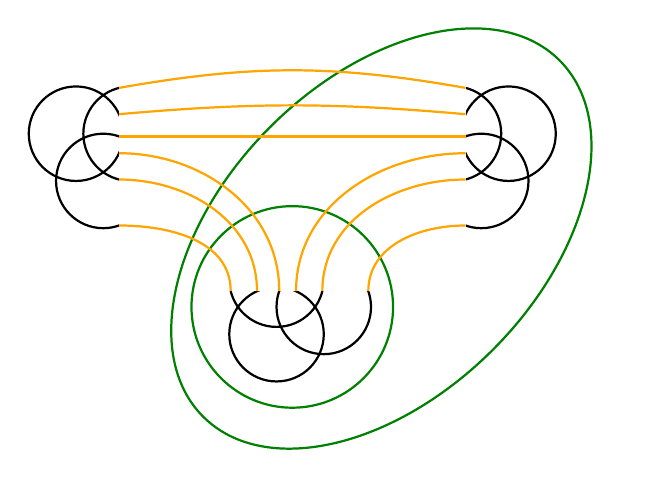
\begin{tikzpicture}[scale=.4]

    % Define the base 3-circle Venn diagram as a reusable macro
    \def\venndiagram{
        \draw[thick] (-90:1) circle (1.5);
        \draw[thick] (30:1) circle (1.5);
        \draw[thick] (150:1) circle (1.5);
    }

    % Define the exact symmetric cut points at x = 0.5 
    % Ordered from top to bottom
    \def\cutX{0.5}
    \def\yA{1.9546} % C2 Top
    \def\yB{1.1197} % C3 Top
    \def\yC{0.4142} % C1 Top
    \def\yD{-0.1197} % C3 Bottom
    \def\yE{-0.9546} % C2 Bottom
    \def\yF{-2.4142} % C1 Bottom

    % --- LEFT DIAGRAM ---
    % Cut on the right side, strands point RIGHT
    \begin{scope}[xshift=-6cm, yshift=0cm]
        \venndiagram
        \fill[white] (\cutX, -3) rectangle (3, 3);
        
        \coordinate (L1) at (\cutX, \yA);
        \coordinate (L2) at (\cutX, \yB);
        \coordinate (L3) at (\cutX, \yC);
        \coordinate (L4) at (\cutX, \yD);
        \coordinate (L5) at (\cutX, \yE);
        \coordinate (L6) at (\cutX, \yF);
    \end{scope}

    % --- RIGHT DIAGRAM ---
    % Mirrored, cut on the left side, strands point LEFT
    \begin{scope}[xshift=6cm, yshift=0cm, xscale=-1]
        \venndiagram
        \fill[white] (\cutX, -3) rectangle (3, 3);
        
        \coordinate (R1) at (\cutX, \yA);
        \coordinate (R2) at (\cutX, \yB);
        \coordinate (R3) at (\cutX, \yC);
        \coordinate (R4) at (\cutX, \yD);
        \coordinate (R5) at (\cutX, \yE);
        \coordinate (R6) at (\cutX, \yF);
    \end{scope}

    % --- MIDDLE DIAGRAM ---
    % Shifted down and rotated 90 degrees.
    % The cut is now on TOP. Strands point UP.
    % Due to rotation mapping (x,y) -> (-y,x), M1 is now the leftmost point, M6 rightmost.
    \begin{scope}[xshift=0cm, yshift=-5cm, rotate=90]
        \venndiagram
        \fill[white] (\cutX, -3) rectangle (3, 3);
        
        \coordinate (M1) at (\cutX, \yA);
        \coordinate (M2) at (\cutX, \yB);
        \coordinate (M3) at (\cutX, \yC);
        \coordinate (M4) at (\cutX, \yD);
        \coordinate (M5) at (\cutX, \yE);
        \coordinate (M6) at (\cutX, \yF);
    \end{scope}

    % --- NEW ENCLOSING CURVE ---
    % Enclosing the middle copy as requested
    \draw[Green, thick] (0, -5) circle (3.2cm);

    \draw[Green, thick, rotate=45] (0,-4) ellipse (8cm and 5cm);


    % --- CONNECTING CURVES ---
    % in/out angles control tangents perfectly to avoid cusps and tangles.

    % 1. Left (Upper) to Right (Upper) - Arching over the top
    \draw[Orange, thick] (L1) to[out=10, in=170] (R1);
    \draw[Orange, thick] (L2) to[out=5,  in=175] (R2);
    \draw[Orange, thick] (L3) to[out=0,  in=180] (R3);

    % 2. Left (Lower) to Middle (Left side)
    % Leaves L pointing Right (out=0), Arrives M from above (in=90)
    % Sorted by width/height so they perfectly nest inside each other
    \draw[Orange, thick] (L4) to[out=0, in=90] (M3);
    \draw[Orange, thick] (L5) to[out=0, in=90] (M2);
    \draw[Orange, thick] (L6) to[out=0, in=90] (M1);

    % 3. Right (Lower) to Middle (Right side)
    % Leaves R pointing Left (out=180), Arrives M from above (in=90)
    \draw[Orange, thick] (R4) to[out=180, in=90] (M4);
    \draw[Orange, thick] (R5) to[out=180, in=90] (M5);
    \draw[Orange, thick] (R6) to[out=180, in=90] (M6);

\end{tikzpicture}